%% Hand-drawn (TikZ) overview of the pipeline for Section III. NOT generated by
%% analysis/ -- edit by hand. Library-free on purpose (core tikz only) so main.tex
%% needs no \usetikzlibrary. Tool name goes through \tool (anonymity build).
%% Iteration notes + an image-model prompt for a raster variant: see
%% pipeline-image-prompt.md next to this file.
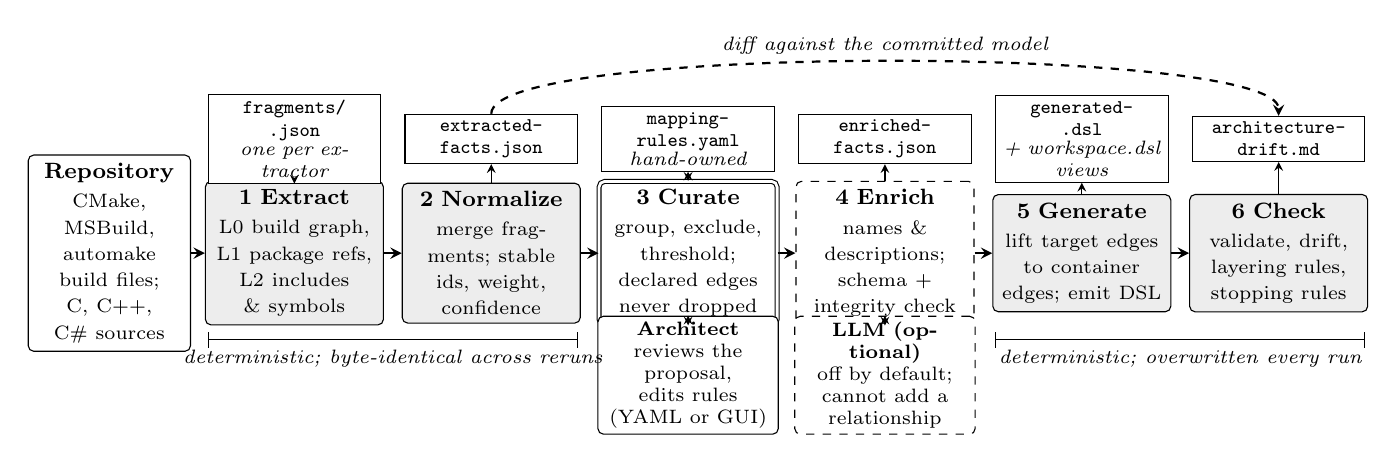
\begin{tikzpicture}[x=1cm,y=1cm,
  stage/.style={draw, rounded corners=2pt, fill=black!7, minimum height=1.3cm,
                text width=2.05cm, align=center, inner sep=3pt, font=\footnotesize},
  human/.style={stage, fill=white, double, double distance=1pt},
  llm/.style={stage, fill=white, dashed},
  art/.style={draw, fill=white, text width=2.05cm, align=center, inner sep=2pt,
              font=\scriptsize\ttfamily},
  io/.style={draw, rounded corners=2pt, fill=white, minimum height=1.3cm,
             text width=1.85cm, align=center, inner sep=3pt, font=\footnotesize},
  actor/.style={draw, rounded corners=2pt, fill=white, text width=2.15cm, align=center,
                inner sep=2pt, font=\scriptsize},
  lane/.style={font=\scriptsize\itshape, align=center},
  flow/.style={->, >=stealth, thick},
  ]
  % ---- inputs --------------------------------------------------------------
  \node[io] (in) at (1.0,0) {\textbf{Repository}\\[1pt]
    {\scriptsize CMake, MSBuild, automake build files; C, C++, C\# sources}};
  % ---- stages --------------------------------------------------------------
  \node[stage] (s1) at (3.35,0)  {\textbf{1 Extract}\\[1pt]
    {\scriptsize L0 build graph, L1 package refs, L2 includes \& symbols}};
  \node[stage] (s2) at (5.85,0)  {\textbf{2 Normalize}\\[1pt]
    {\scriptsize merge fragments; stable ids, weight, confidence}};
  \node[human] (s3) at (8.35,0)  {\textbf{3 Curate}\\[1pt]
    {\scriptsize group, exclude, threshold; declared edges never dropped}};
  \node[llm]   (s4) at (10.85,0) {\textbf{4 Enrich}\\[1pt]
    {\scriptsize names \& descriptions; schema + integrity check}};
  \node[stage] (s5) at (13.35,0) {\textbf{5 Generate}\\[1pt]
    {\scriptsize lift target edges to container edges; emit DSL}};
  \node[stage] (s6) at (15.85,0) {\textbf{6 Check}\\[1pt]
    {\scriptsize validate, drift, layering rules, stopping rules}};
  \draw[flow] (in) -- (s1);
  \draw[flow] (s1) -- (s2);
  \draw[flow] (s2) -- (s3);
  \draw[flow] (s3) -- (s4);
  \draw[flow] (s4) -- (s5);
  \draw[flow] (s5) -- (s6);
  % ---- artifacts (what each stage writes) ---------------------------------
  \node[art] (a1) at (3.35,1.45)  {fragments/\\*.json\\[-1pt]{\rmfamily\itshape one per extractor}};
  \node[art] (a2) at (5.85,1.45)  {extracted-\\facts.json};
  \node[art] (a3) at (8.35,1.45)  {mapping-\\rules.yaml\\[-1pt]{\rmfamily\itshape hand-owned}};
  \node[art] (a4) at (10.85,1.45) {enriched-\\facts.json};
  \node[art] (a5) at (13.35,1.45) {generated-\\*.dsl\\[-1pt]{\rmfamily\itshape + workspace.dsl views}};
  \node[art] (a6) at (15.85,1.45) {architecture-\\drift.md};
  \foreach \i in {1,2,4,5,6} { \draw[->, >=stealth] (s\i.north) -- (a\i.south); }
  \draw[<->, >=stealth] (s3.north) -- (a3.south);
  % drift compares the fresh facts with the committed model
  \draw[flow, dashed] (a2.north) .. controls +(0,0.9) and +(0,0.9) .. (a6.north)
    node[midway, above=-1pt, lane] {diff against the committed model};
  % ---- who is in the loop --------------------------------------------------
  \node[actor] (arch) at (8.35,-1.55) {\textbf{Architect}\\ reviews the proposal,\\ edits rules (YAML or GUI)};
  \node[actor, dashed] (model) at (10.85,-1.55) {\textbf{LLM (optional)}\\ off by default;\\ cannot add a relationship};
  \draw[<->, >=stealth] (s3.south) -- (arch.north);
  \draw[<->, >=stealth, dashed] (s4.south) -- (model.north);
  \draw[|-|] (2.25,-1.1) -- (6.95,-1.1) node[midway, below, lane] {deterministic; byte-identical across reruns};
  \draw[|-|] (12.25,-1.1) -- (16.95,-1.1) node[midway, below, lane] {deterministic; overwritten every run};
\end{tikzpicture}
